\section*{Assignment 02: Network Effects and Launch Strategy}
\addcontentsline{toc}{section}{Assignment 02: Network Effects and Launch Strategy}

\subsection*{Network effects mapped explicitly}
I followed \citet{Choudary2016}'s three step loop mapping exercise to keep the network effects honest. Step one \textbf{defines the core interaction}: a vetted organisation posts a scoped brief, curated students respond, and both sides commit to a sprint. Step two \textbf{specifies reinforcing signals}. The cross side loop grows when visible success stories and quick responses reassure the next wave of users. Student same side effects stem from peer endorsements and a ritual where alumni leave short Loom videos once a sprint ends, echoing Lecture~4's point that \textit{social proof reduces cold start friction} \citep{Lecture04}. Organisation same side effects emerge when NGOs see comparable peers succeeding, so I pencilled monthly showcase calls. Finally \textbf{the data loop records skills used}, hours invested, and satisfaction scores, upgrading the matching algorithm each cycle and nudging SkillSync toward the orchestrator pattern \citep{Reillier2017}.

\subsection*{Solving the penguin problem}
To break the mutual hesitation \citet{HagiuWright2013} warn about, the launch plan recruits two anchor NGOs already comfortable mentoring students. They become the first proof points and agree to share testimonials. Parallel to that, I recruit about 40 students through faculty recommendations, student societies, and the course Slack so quality stays predictable. A fast onboarding script walks both sides through the first mission: Manually review briefs, pair mentors, and host a kickoff call. Students receive travel stipends for the first sprint funded by a faculty innovation grants, while NGOs get a temporary fee waiver that expires after two successful projects, following \citet{FarrellSaloner1986}'s logic on \textit{introductory pricing}.

Communication routines are scripted in advance. Weekly check-ins and a shared calendar keep the first ten projects on track; we log every difficult point and feed it into a FAQ public for all. With inspiration from Lecture~4 guidance: \textit{when seeding a platform, design commitment devices that keep early adopters active long enough for loops to form} \citep{Lecture04}. I also plan a backup: if a project fails mid sprint, SkillSync deploys a standby student pair from the founding 40 students, within forty eight hours, so organisations trust us despite hiccups.

\subsection*{Launch measurements and decision rules}
Because there is no live \textit{product} yet, my reflections read \textit{pre mortem}. I focus on \textbf{three metrics}. Value measures \textbf{minutes from signup to first action}; if it exceeds 30 minutes the team must simplify the process. \textbf{Match completion rate}, tracks how many pairs finish within scope; a dip below 70\% triggers a session (With root cause). Early net promoter score captures qualitative trust; scores below plus twenty prompt follow up interviews. These numbers come from \citet{ShapiroVarian1999}'s advice to \textit{anchor monetisation on observed value} and from Lecture~5's insistence that early experiments should move one behaviour at a time \citep{Lecture05}. Figure~\ref{fig:application-flow} visualises the guided student flow that underpins these metrics.

\begin{figure}[H]
  \centering
  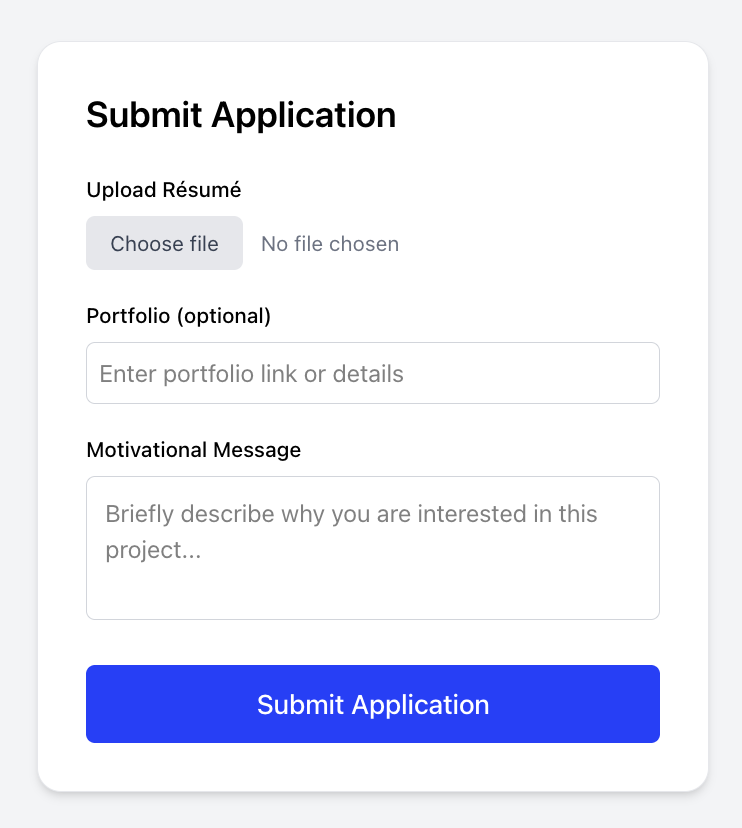
\includegraphics[width=0.85\linewidth]{figures/Student-Submission.png}
  \caption{Student application flow mock up with guided pitch submission.}
  \label{fig:application-flow}
\end{figure}

I mirror the journey for organisations in Assignment~03. The idea is to choreograph both sides simultaneously so that once the early subsidies phase out, the playbook already embeds trust instead of improvised fixes.
